\chapter{Technical Specification}
\section{Protocol}

The protocol of our signing service consists of five main phases:

\begin{itemize}
	\item Pre-Login
	\item Login
	\item Post-Login
	\item Signature Generation
	\item Signature Verification
\end{itemize}

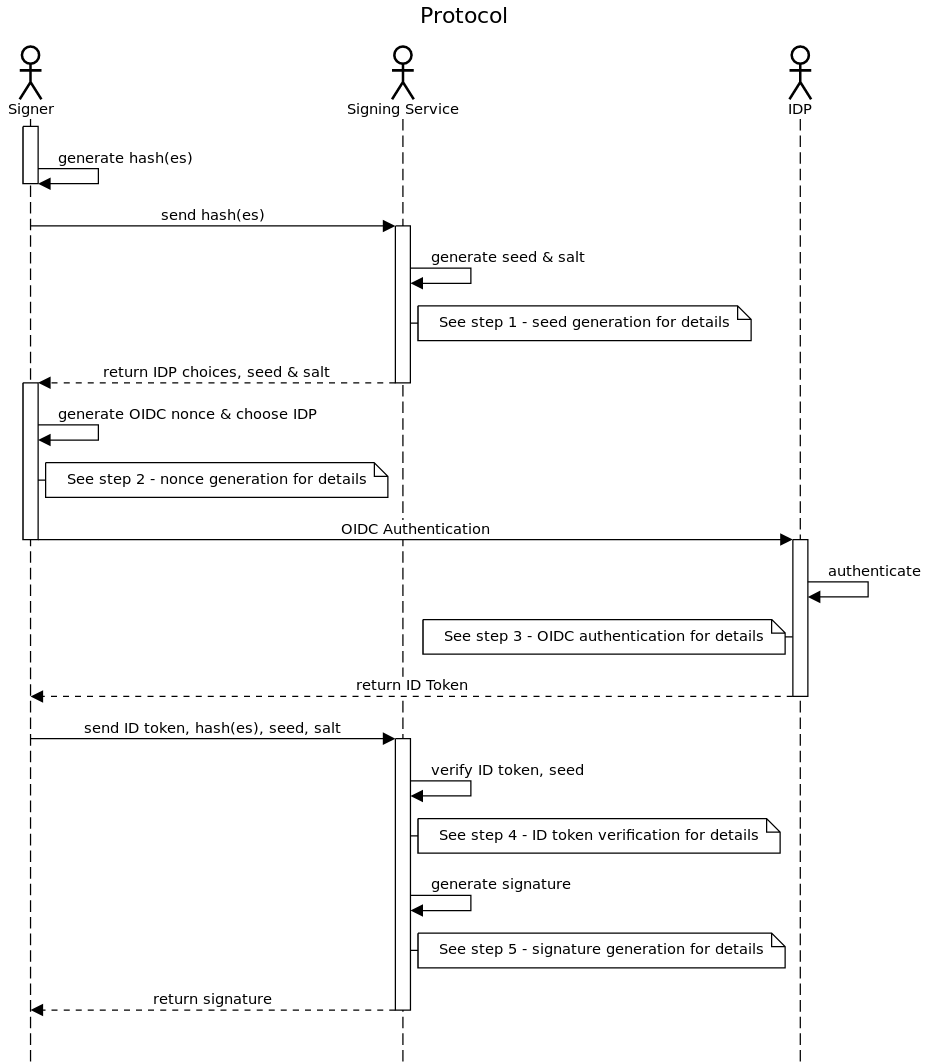
\includegraphics[scale=0.5]{images/protocol_signature_generation_high_level.png}

\subsection{Pre-Login}
In this phase the signer provides a list of hashes to signing service. 

Afterwards the signing service generates a random seed value. This seed and a secret only known to the server will be used to calculate the key that will be used to generate a \gls{HMAC} of the sorted list of hashes. The \gls{HMAC} will be used as a salt to the hashes in the \gls{OIDC} nonce. The key consists simply of appending the secret to the seed.

Purpose of the salt:
The salt is used to protect the hashes in the \gls{OIDC} nonce both from the \gls{IDP}, so that it doesn't know if two people sign the same document(s) and the receiver of the signature as it needs a list of all hashes that have been signed together to verify the signature.

Purpose of the seed:
The seed is used as a \gls{CSRF} protection mechanism without keeping any state on the server.
If no seed is used for generating the salt, the signing server needs to keep it in memory and attach it to the users session in order to verify if the hashes or the salt weren't replaced while generating the \gls{OIDC} nonce.
If the signing server doesn't verify this it would enable clients/attackers to skip the Pre-Login step.

The server than returns a list of \gls{IDP} choices, the seed and the salt to the client.

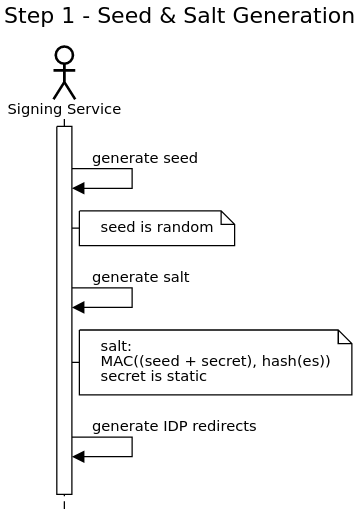
\includegraphics[scale=0.5]{images/protocol_step1_seed_generation.png}

\subsection{Login}
The client generates the nonce used for the \gls{OIDC} request which consists of the Hash of the sorted list of \gls{HMAC}s of the Hashes with the returned salt used as key. 
Next the client chooses an \gls{IDP} and adds the nonce to the request parameters and then follows the link. At the \gls{IDP} the client signs in and gets an ID token back.

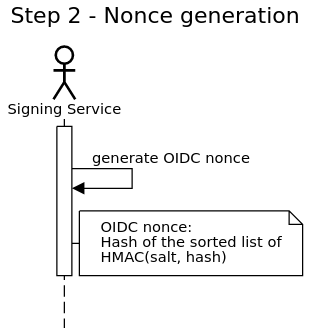
\includegraphics[scale=0.5]{images/protocol_step2_nonce_generation.png}

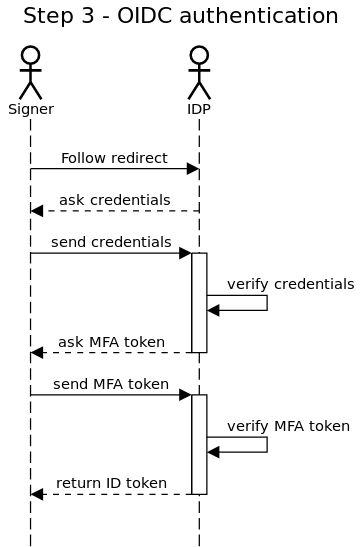
\includegraphics[scale=0.5]{images/protocol_step3_oidc_authentication.png}

\subsection{Post-Login}
The client sends the ID token, the list of hashes, the seed and the salt to the signing service. The signing service then proceeds to verify the salt, OIDC nonce and ID token.
After verifying the salt, the seed is not used anymore.
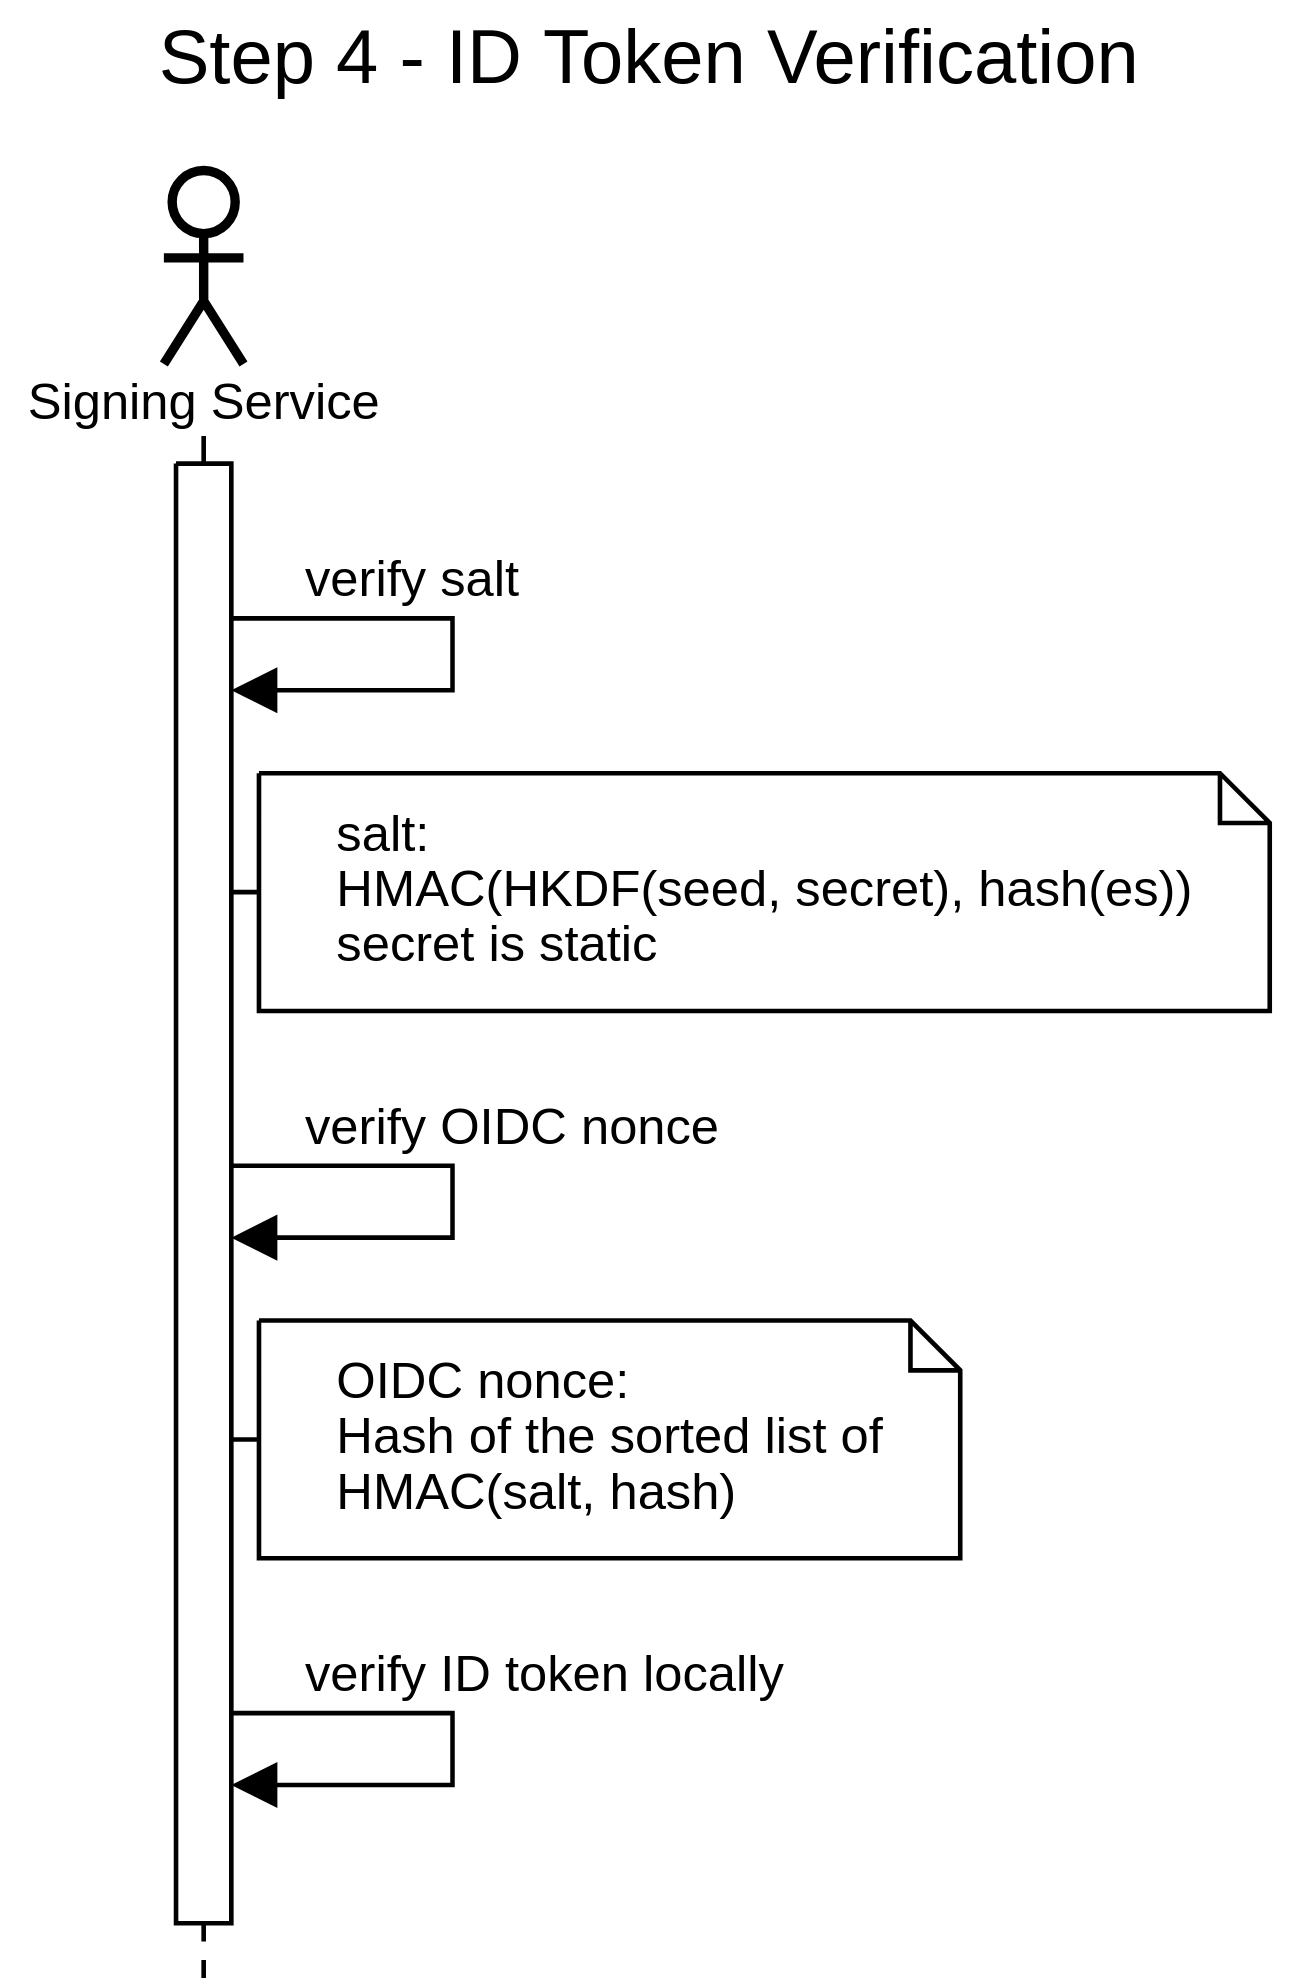
\includegraphics[scale=0.5]{images/protocol_step4_id_token_verification.png}

\subsection{Signature Generation}
The signing server requests a new signing key from the hsm, which will generate a private key and return a \gls{CSR}.
The \gls{CSR} is sent to the \gls{CA} where it will be signed and the signed certificate is returned.
Each hash is then submitted to the \gls{HSM} in order to be signed by the generated key.

For each hash an intermediate signature file consisting of the signed hash, the ID token, the salt and a sorted list of all other salted hashes.
The hash of this file is sent to a \gls{TSA} where a signed timestamp will be created and returned.
The signed timestamp and all the certificate chains and ocsp responses of the involved parties will be added to signature file, which is then returned to the user.

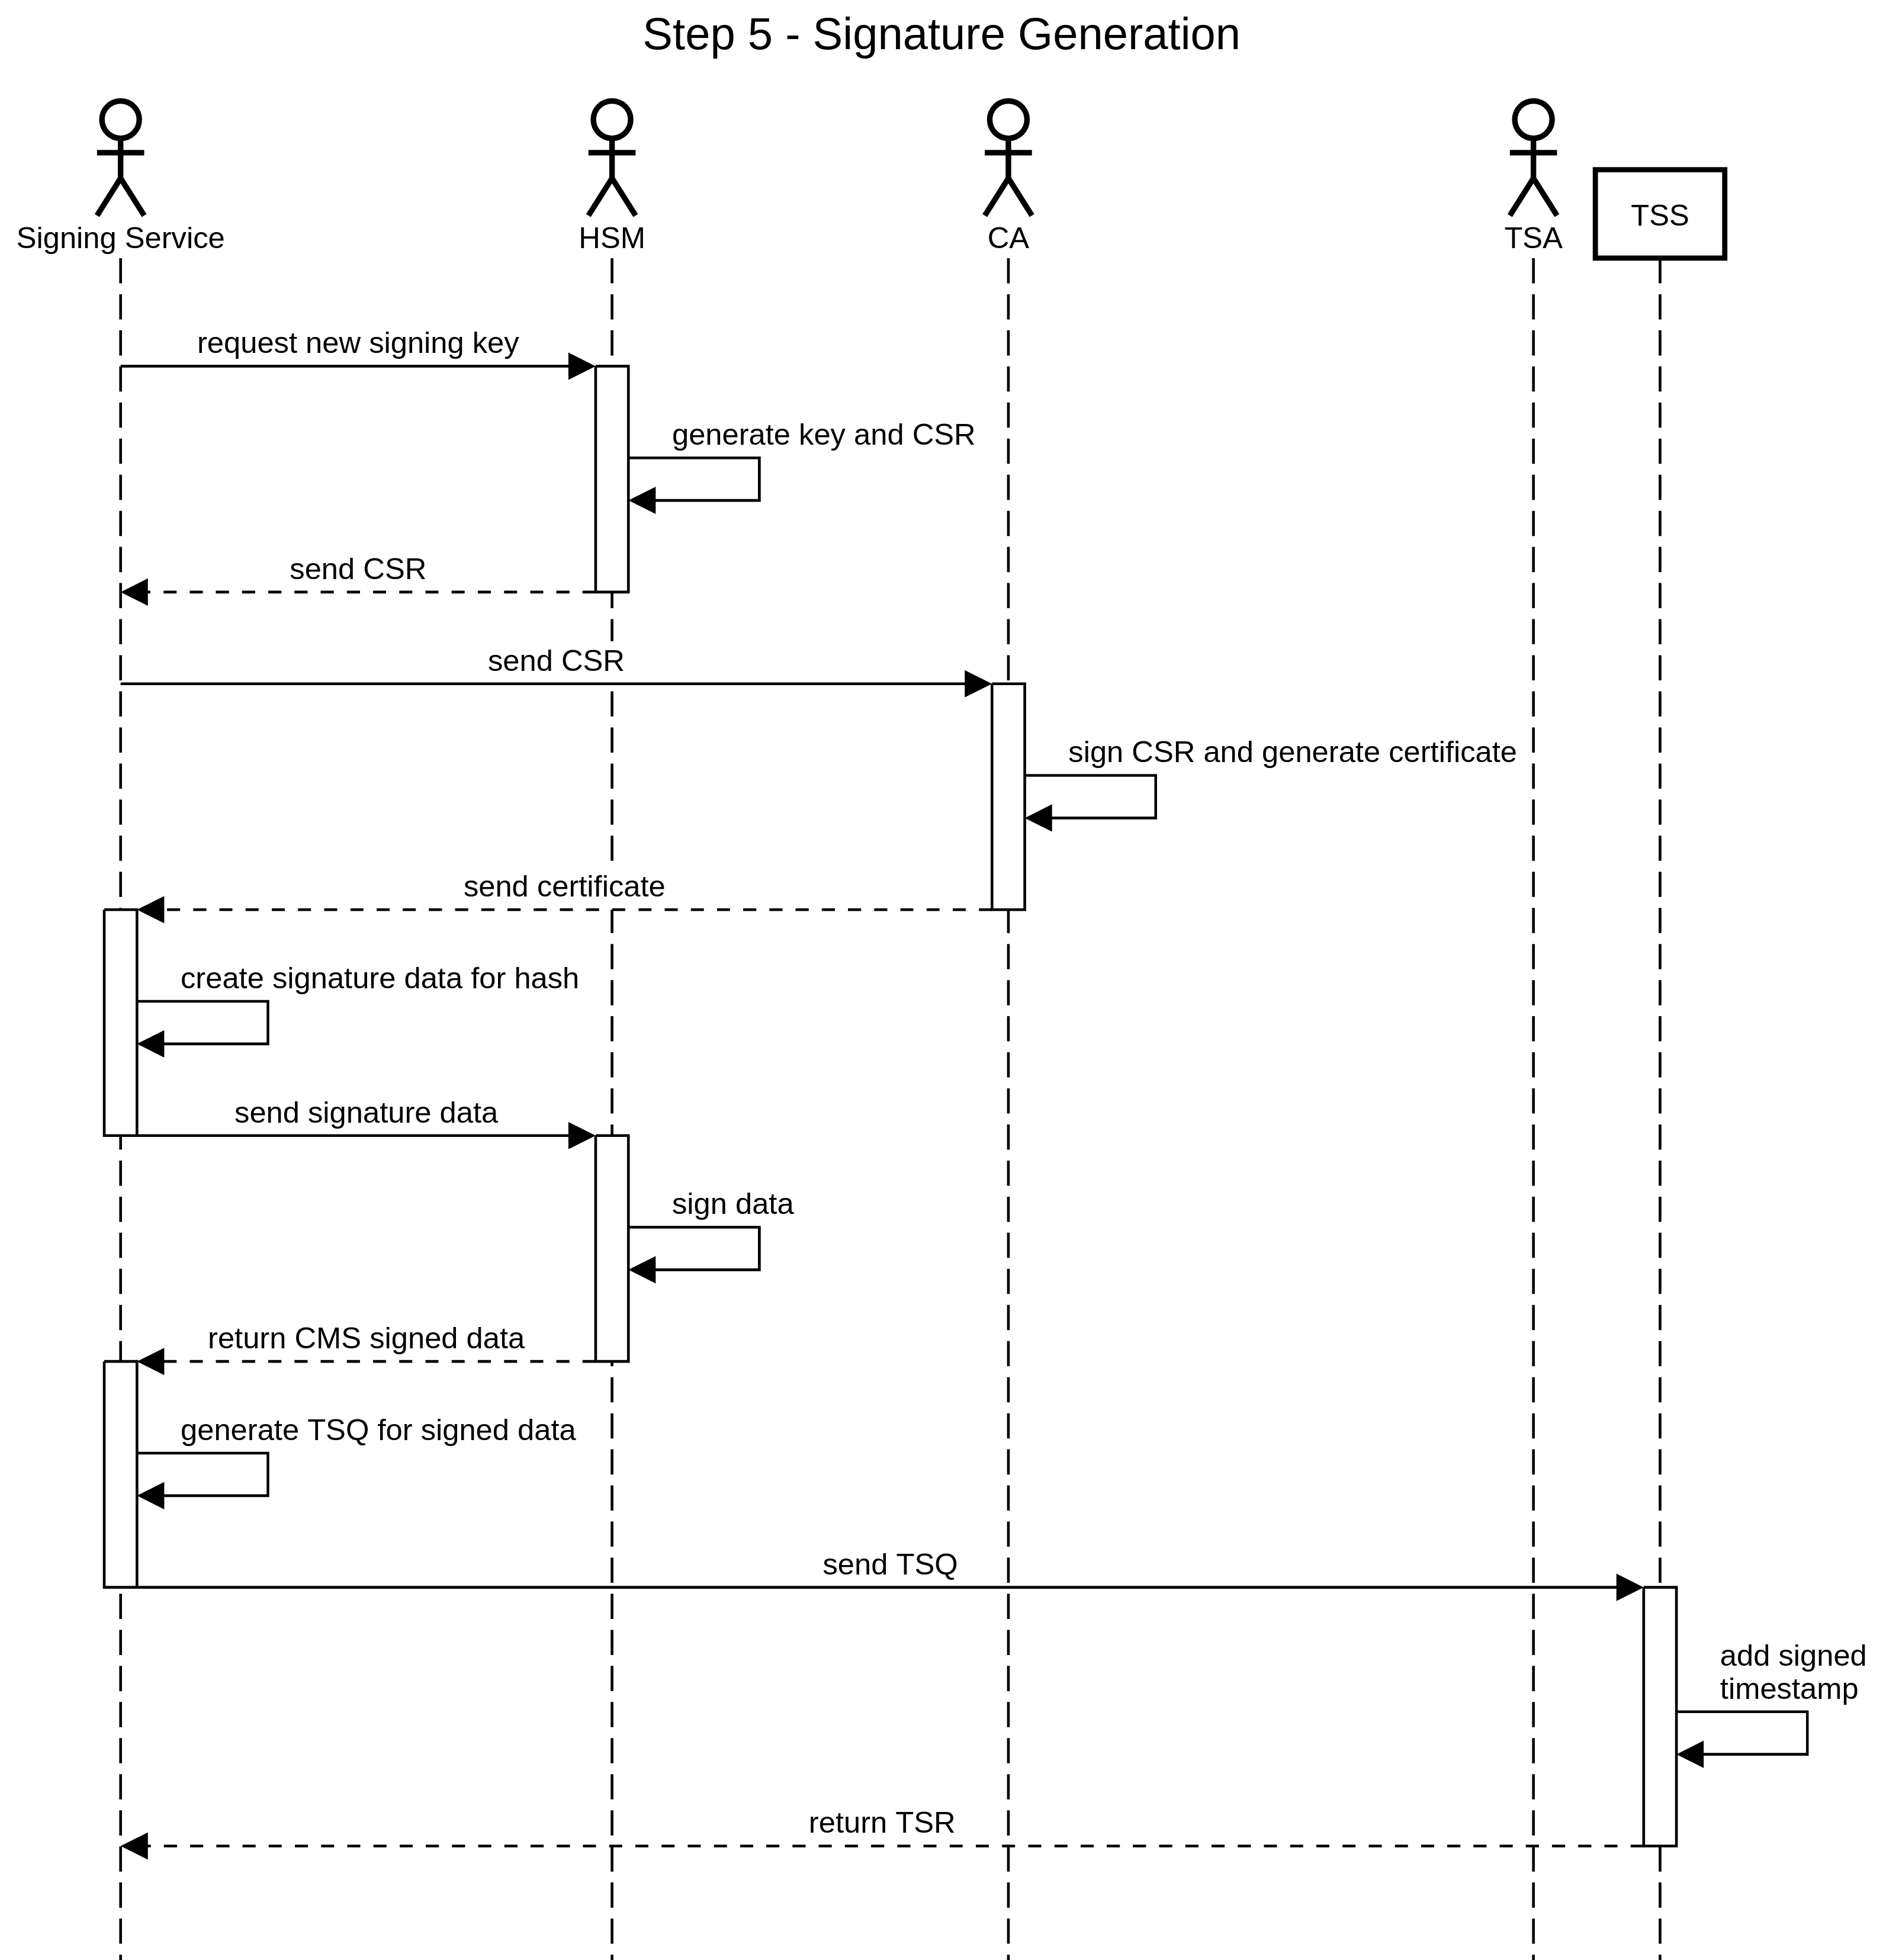
\includegraphics[scale=0.45]{images/protocol_step5_signature_generation.png}

\subsection{Signature Verification}
To verify a signature the verifier first needs to verify the signed timestamp(s) and their respective ca chains.
The signature then can be verified.
Next the certificate chain for the signing certificate needs to be verified.
Then the certificate chain for the ID token needs to be verified.
The ID token itself also needs to be verified.
The included hash needs to be salted and then together with the sorted list of salted hashes hashed.
The result must be the same as the nonce in the ID token.
At last the hash of the document MUST match the included hash.

\section{REST API}
Endpoints:

\begin{tabular}{|l|l|l|}
	\hline
	Endpoint & Method & Description \\ \hline
	/api/v1/hashes & POST & send hashes to generate nonce \\ \hline
	/api/v1/login & POST & get oidc providers \\ \hline
	/api/v1/sign & POST & sign hashes \\ \hline
	/api/v1/signatures & GET & retrieve list of all signatures for current session \\ \hline
	/api/v1/signatures/:hash & GET & retrieve signature \\ \hline
\end{tabular}

\subsection{hashes}
Input:

\begin{tabular}{|l|l|l|l|}
	\hline
	Parameter & Presence & Type & Description \\ \hline
	hashes & MANDATORY & list(string) & Hashes of the documents to be signed \\ \hline
\end{tabular}

Output:

\begin{tabular}{|l|l|l|l|}
	\hline
	Parameter & Presence & Type & Description \\ \hline
	nonce & MANDATORY & string & Nonce to use for generating to OIDC nonce in the token \\ \hline
\end{tabular}

Sample Request:
\begin{lstlisting}[caption={hashes request}, captionpos=b, language=JavaScript, label={lst:hashesrequest}]
POST /api/v1/hashes HTTP/1.1
Host: service.example.org
Content-Type: application/json

{
  "hashes": [
  "e8a96e6203b9c0df058ba862abc63d9c520157faef6d5d54e54e526b0a85b2be",
  "0b9a7fd3e612061a7fe6d834e102a143170f33d0e8c5a8eb79416aa3eb53c0d6"
  ]
}
\end{lstlisting}

Sample Response:
\begin{lstlisting}[caption={hashes response}, captionpos=b, language=JavaScript, label={lst:hashesresponse}]
HTTP/1.1 201 Created
Content-Type: application/json

{
  "nonce": "test1234"
}
\end{lstlisting}

\subsection{login}
Input:

\begin{tabular}{|l|l|l|l|}
	\hline
	Parameter & Presence & Type & Description \\ \hline
	nonce & MANDATORY & string & Nonce to use for retrieving the OIDC token \\ \hline
\end{tabular}

Output:

\begin{tabular}{|l|l|l|l|}
	\hline
	Parameter & Presence & Type & Description \\ \hline
	providers & MANDATORY & dictionary[string]url & List of providers with the redirect url \\ \hline
\end{tabular}

Sample Request:
\begin{lstlisting}[caption={login request}, captionpos=b, language=JavaScript, label={lst:loginrequest}]
POST /api/v1/login HTTP/1.
Host: service.example.org
Content-Type: application/json

{
  "nonce": "6cd7ef99e5e79d68d681e5d097b7f805381c4d013152fa3f26d06bd728ae49fa"
}
\end{lstlisting}

Sample Response:

\begin{lstlisting}[caption={login response}, captionpos=b, language=JavaScript, label={lst:loginresponse}]
HTTP/1.1 200 OK
Content-Type: application/json

{
  "providers": {
    "SwissID": "https://...&nonce=6cd7ef99e5e79d68d681e5d097b7f805381c4d013152fa3f26d06bd728ae49fa",
    "Google": "https://...&nonce=6cd7ef99e5e79d68d681e5d097b7f805381c4d013152fa3f26d06bd728ae49fa"
  }
}
\end{lstlisting}

\subsection{sign}
Input:

\begin{tabular}{|l|l|l|l|}
	\hline
	Parameter & Presence & Type & Description \\ \hline
	idtoken & MANDATORY & string & OIDC ID token \\ \hline
	nonce & MANDATORY & string & Nonce to use for generating to OIDC nonce in the token \\ \hline
	hashes & MANDATORY & list(string) & Hashes of the documents to be signed \\ \hline
\end{tabular}

Output:

\begin{tabular}{|l|l|l|l|}
	\hline
	Parameter & Presence & Type & Description \\ \hline
	result & MANDATORY & bool & Status of the signing (true = success, false = failure) \\ \hline
\end{tabular}

Sample Request:
\begin{lstlisting}[caption={sign request}, captionpos=b, language=JavaScript, label={lst:signrequest}]
POST /api/v1/sign HTTP/1.
Host: service.example.org
Content-Type: application/json

{
  "idtoken": {...},
  "nonce": "test1234",
  "hashes": [
    "e8a96e6203b9c0df058ba862abc63d9c520157faef6d5d54e54e526b0a85b2be",
    "0b9a7fd3e612061a7fe6d834e102a143170f33d0e8c5a8eb79416aa3eb53c0d6"
  ]
}
\end{lstlisting}

Sample Response:

\begin{lstlisting}[caption={sign response}, captionpos=b, language=JavaScript, label={lst:signresponse}]
HTTP/1.1 201 Created
Content-Type: application/json

{
  "result": true
}
\end{lstlisting}

\subsection{signatures}
Output:

\begin{tabular}{|l|l|l|l|}
	\hline
	Parameter & Presence & Type & Description \\ \hline
	hashes & MANDATORY & list(string) & hashes that were signed \\ \hline
\end{tabular}

Sample Request:

\begin{lstlisting}[caption={signatures request}, captionpos=b, language=JavaScript, label={lst:signaturesrequest}]
GET /api/v1/signatures HTTP/1.
Host: service.example.org
Content-Type: application/json
\end{lstlisting}

Sample Response:

\begin{lstlisting}[caption={signatures response}, captionpos=b, language=JavaScript, label={lst:signaturesresponse}]
HTTP/1.1 200 OK
Content-Type: application/json

{
  "hashes": [
    "e8a96e6203b9c0df058ba862abc63d9c520157faef6d5d54e54e526b0a85b2be",
    "0b9a7fd3e612061a7fe6d834e102a143170f33d0e8c5a8eb79416aa3eb53c0d6"
  ]
}
\end{lstlisting}

\subsection{signatures/:hash}
Input:

\begin{tabular}{|l|l|l|l|}
	\hline
	Parameter & Presence & Type & Description \\ \hline
	hash & MANDATORY & string & hash that was signed \\ \hline
\end{tabular}

Output:

\begin{tabular}{|l|l|l|l|}
	\hline
	Parameter & Presence & Type & Description \\ \hline
	signature & MANDATORY & binary & base64 encoded signature for the requested hash \\ \hline
\end{tabular}

Sample Request:

\begin{lstlisting}[caption={signature request}, captionpos=b, language=JavaScript, label={lst:signaturerequest}]
GET /api/v1/signatures/e8a96e6203b9c0df058ba862abc63d9c520157faef6d5d54e54e526b0a85b2be HTTP/1.
Host: service.example.org
Content-Type: application/json
\end{lstlisting}

Sample Response:

\begin{lstlisting}[caption={signature response}, captionpos=b, language=JavaScript, label={lst:signatureresponse}]
HTTP/1.1 200 OK
Content-Type: application/json

{
  "signature": "IyMjIFJFU1QgQVBJIFNwZWNpZmljYXRpb24gU2NyYXRjaHBhZAoKIyMjIyBQcmUtQXV0aCBlbmRw...b2ludCAKIyMjIyMgRW5kcG9pbnQKYGBgUE9TVCAvYXBpL3YxL3NpZ25gYGAK"
}
\end{lstlisting}

\section{Signature File Format}
TODO
\subsection{Long-Term Validation}
\gls{LTV} allows for the validation of signatures long after the document was signed~\cite{etsipades}.

We need \gls{LTV} for two main reasons:
\begin{enumerate}
    \item Imagine if the \gls{CA} were revoked that was used for the signatures: all signatures created using the same \gls{CA} would become invalid instantly, making countless documents, constracts and the like unverifiable.
    \item Extending the validity of the signature beyond the lifetime of the \gls{CA} used to sign it, for signatures that need to remain valid and verifiable for a very long time.
\end{enumerate}
In order for us to achieve this, all required elements for signature validation must be embedded into the signature file.
Without the addition of these elements, a signature can only be validated for a limited time.
This limitation occurs because the \gls{CA}s eventually expire, or get revoked.
Once the \gls{CA} certificate has expired, the issuing authority is no longer responsible for providing the revocation status information on that certificate.
Without the confirmed revocation status information on the signing keys, the signature cannot be validated.

To overcome this limitation, the following information has to be embedded into the signature:
\begin{enumerate}
    \item A timestamp on the signature
    \item The signing certificate
    \item The certificates used and their revocation status (\gls{OCSP} and \gls{CRL})
    \item An archive timestamp of the previous content
\end{enumerate}

The archive timestamp establishes the date in which the information collected was issued.
Provided the archive timestamp is valid,
we can be sure that the revocation information was issued at that time,
and check the validity of the signing certificate and the \gls{CA} certificate chain.
Thus we can be certain that it was not revoked at the point in time the document was signed.
This allows us to extend the validity of the signature past the expiration time of the \gls{CA}.

However, this does not extend the validity of the signature indefinitely,
it merely extends the expiration until the expiration time of the timestamping authority's certificate.

For many cases this may be enough, but it doesn't quite allow for long-time archival yet.
When the timestamping certificates' expiration is impending,
the signature expiration time has to be extended by adding another timestamp signed by a \gls{CA} not yet close to expiration.
This re-stamping has to be repeated periodically in order to keep the signature valid and verifiable.
This allows for near-indefinite archival.

